\documentclass[a4paper]{article}

% Linguagem
\usepackage[utf8]{inputenc}
\usepackage[portuguese]{babel}
\usepackage[T1]{fontenc}

% Pacotes matemáticos
\usepackage{amsmath}
\usepackage{amsfonts}
\usepackage{amssymb}
\usepackage{graphicx}

% Fontes e identaçãp
\usepackage{setspace}                   % espaçamento flexível
\usepackage{indentfirst}                % indentação do primeiro parágrafo
\usepackage[fixlanguage]{babelbib}
\usepackage[font=small,format=plain,labelfont=bf,up,textfont=it,up]{caption}

% Pacotes para cores e modelos
\usepackage[a4paper,top=3.0cm,bottom=2.0cm,left=3.0cm,right=2.0cm]{geometry} \usepackage[usenames,svgnames,dvipsnames]{xcolor}
\usepackage[pdftex,plainpages=false,pdfpagelabels,pagebackref,
            colorlinks=true,citecolor=DarkGreen,linkcolor=DarkRed,
            urlcolor=DarkRed,filecolor=DarkGreen,
            bookmarksopen=true]{hyperref}

% Pacotes para itens
\usepackage{calc}  
\usepackage{enumitem}  

\title  {Projeto de Laboratório de Programação II - Fase 2}
\author {Karina Suemi, Vinícius Silva, Renato Cordeiro}
\date   {}

%%%%%%%%%%%%%%%%%%%%%%%%%%%%%%%%%%%%%%%%%%%%%%%%%%%%%%%%%%%%%%%%%%%%%%%%

\begin{document}

\maketitle

\bigskip
\bigskip
\bigskip
\bigskip

{\textcolor{NavyBlue}{\Huge{....... MANUAL DO USUÁRIO .......}}


\newpage

     
{\textcolor{NavyBlue}{\LARGE JOGO }

\bigskip

O  jogo consiste  em programar uma  série de 
robôs para batalharem, num estilo de RTS 2x2.
Para  tanto,  os robôs devem  ter suas ações 
programadas. Eles irão executá-las até que o 
jogo acabe ou sejam destruídos.

Nesta fase do desenvolvimento, a programação 
deve  ser  feita   em  linguagem  *Assembly*,
desenvolvida  especialmente  para  a máquina 
virtual  em *Java*. 

Os programas devem  ser criados com extensão 
*.asm*.   Exemplos   estão   disponíveis  no 
diretório `test/` junto ao código-fonte. 



\bigskip
\bigskip
\bigskip
\bigskip


{\textcolor{NavyBlue}{\LARGE INSTALAÇÃO }
                
\bigskip
                                            
\textcolor{NavyBlue}{-- 1º PASSO --}

Antes de mais nada, verifique se seu computador possui
o Ant instalado, caso não possua, faça o seguinte:

\begin{enumerate}
	\item Abra o terminal

	\item Digite no terminal: \$: sudo apt-get -u install ant
\end{enumerate}

\bigskip



\textcolor{NavyBlue}{-- 2º PASSO --}

Instalação do ivy:

\begin{enumerate}
	\item Abra o terminal

	\item Entre na pasta (MAC0242-PROJECT)

	\item Digite: \$: sudo bash install\_ivy.bash

	\item E em seguida, digite: \$: ln -s -T /usr/share/java/ivy.jar /usr/share/ant/lib/ivy.jar

\end{enumerate}

\bigskip


\textcolor{NavyBlue}{-- 3º PASSO --}

Para compilar o jogo:

\begin{enumerate}
	\item Ainda com o terminal aberto

	\item Entre na pasta onde está localizado o arquivo do jogo (MAC0242-PROJECT)

	\item Digite \$: ant
\end{enumerate}

\bigskip



\textcolor{NavyBlue}{-- 4º PASSO --}

E para iniciar o jogo: 

\begin{enumerate}                                            
	\item Continuar no terminal
 	\item Digite : \$ \textit{ java -jar dist/MAC0242-Project.jar programa\_jogador\_1 programa\_jogador\_2} 
\end{enumerate}

\bigskip


\newpage %%%%%%%%%%%%%%%%%%%%%%%%%%%%%%%%%%%%%%%%%%%%%%%%%

{\textcolor{NavyBlue}{\LARGE Opções}

Você pode escolher várias formas de jogar A Batalha de Robôs,
sendo que cada uma delas envolve um tipo de cenário diferente.
Entre eles temos:

\begin{itemize}
	\item Artical
	\item Tropical
	\item Desertic
	\item Continental
\end{itemize}

Para jogar cada um deles, basta iniciar o programa do seguinte modo:

\begin{itemize}

	\item Artical --> \begin{verbatim}java -jar dist/MAC0242-Project.jar programa\_jogador\_1 programa\_jogador\_2 --artical\end{verbatim}

	\item Tropical --> \begin{verbatim}java -jar dist/MAC0242-Project.jar programa\_jogador\_1 programa\_jogador\_2 --tropical\end{verbatim}

	\item Desertic --> \begin{verbatim}java -jar dist/MAC0242-Project.jar programa\_jogador\_1 programa\_jogador\_2 --desertic\end{verbatim}

	\item Continental --> \begin{verbatim}java -jar dist/MAC0242-Project.jar programa\_jogador\_1 programa\_jogador\_2 --continental\end{verbatim}



\end{itemize}

\bigskip
\bigskip


{\textcolor{NavyBlue}{\LARGE exemplos:}

\bigskip

\begin{figure}[h]
	\centering
    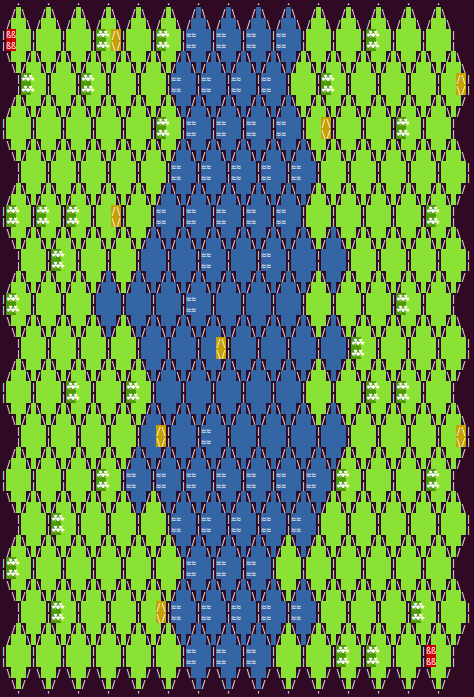
\includegraphics[scale=0.3]{TROPICAL.png}
    \caption{Tropical}
\end{figure}

\bigskip

\begin{figure}[h]
   	\centering
    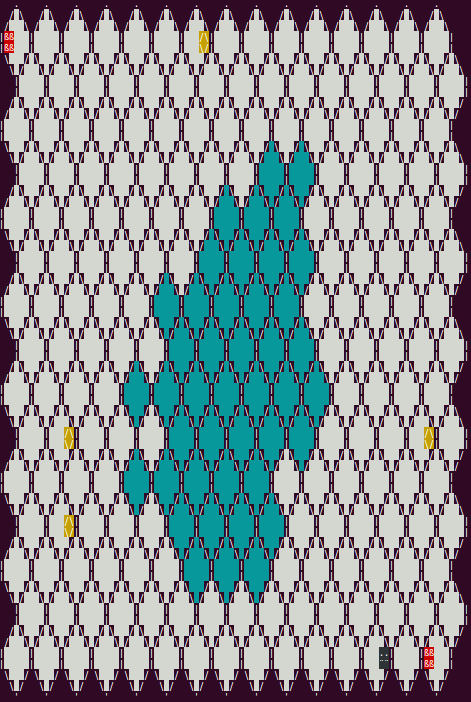
\includegraphics[scale=0.3]{ARTICAL.png}
    \caption{Artical}
\end{figure}

\newpage %%%%%%%%%%%%%%%%%%%%%%%%%%%%%%%%%%%%%%%%%%%%%%

{\textcolor{NavyBlue}{\LARGE Utilitários}
\begin{itemize}
	\item Para utilizar os programas para os 
	robôs, compile-os com:

	\$ \textit {sh reload.sh path/para/o/arquivo.asm}

	\bigskip

	\item E caso queira executar o programa em modo 
	Debugger, digite:

	\$ \textit {java -jar dist/MAC0242-Project.jar }
    	  programa\_jogador\_1 programa\_jogador\_2 -v

	\bigskip
\end{itemize}


{\textcolor{NavyBlue}{\LARGE DOCUMENTAÇÃO }

A   documentação    do   código-fonte   está 
disponível no formato Javadoc e no formato 
de relatório Latex para compreendimento do 
código.

\end{document}
